\chapter{Background Study}
Ants are social insect. These small tiny creatures have survived major extinction level events in the world. They have been evolved millions of years to survive in the worlds. Their strategies to find resources for their survival are fascinating. We ran several experiments on desert harvester ants at the field to observe how they forage. We have selected three different species of harvester Ants to observe their foraging strategies. Those ants are \textit{P. Rugosus}, \textit{P. Desertorum} and \textit{P. Maricopa}. Our goal was to figure out how they find resources from an environment and what is the effect of the distribution of information on their foraging. So we ran experiments on ants. Seeds in the fields are distributed in a donut shape ring. The area of the food distribution is scaled with the colony size of ants. For example, Desertorum was the smallest in colony size (77$\pm$296), so the donut ring radius of food was 1.5 to 3 meters, Rugosus has a colony size of 1712$\pm$174. So the radius of food distribution for Rugosus was in 5-10 meters. The seeds are organized in a power law distribution around the nest.
\section{\label{section:Power Law}Power Law}
In power law distribution of food, seeds are distributed into multiple piles of different pile size. For example, for power rank 5 of power law distribution total number of seeds will be 1024. And it is divided into 4 types of 256 seeds in each type. One large pile of 256 seeds are placed all together in a certain position. Next 256 seeds are divided into 4 equal sizes of 64 seeds and placed around the nest. Next 256 seeds are equally divided into 16 piles of 16 seeds and placed around the nest inside the ring. Rest of the seeds are distributed uniformly around the nest.
\begin{figure}[h]
	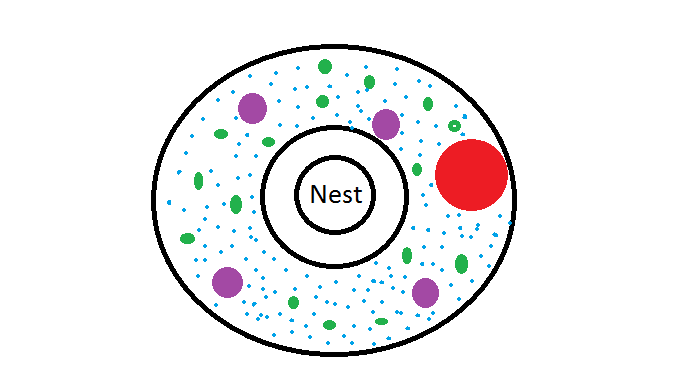
\includegraphics[width=\textwidth]{DonutShape.png}
	\caption{Distribution of Seeds in the field experiment for power law distribution with power rank 5. Red Pile indicates one large pile of 256 seeds. 4 purple piles represent 4 large piles of 64 seeds, Green color represents 16 piles of 16 seeds and blue seeds are 256 random seeds}
\end{figure}
\section{\label{section:CPFA}CPFA}
After the distribution of foods across the nest we observe their collection of seeds. It is observed that ants need longer time to discover the large pile with 256 seeds then the piles with small amount of seeds. But once the seeds are discovered, they started recruiting from the piles. Studies showed that information is transferred among the ants for larger piles with more seeds. We have plotted the collection of seeds from the field experiments and discovered ants walk randomly to collect seeds. Once they get the seed they bring it back to the nest. But if they discover a large food source they share the information with others to recruit from the food source. Once the information is shared more ants come into recruitments and while collecting this food they also share information with other ants. As soon as ants start recruiting from the food source, their foraging rate goes up. But the food source starts losing the number of seeds. As the number of seeds starts decreasing from the food source the recruitment of amount of ants also starts decreasing. Based on this behavior, an algorithm was proposed to simulate the behavior of ants. It is called Central Place Foraging Algorithm(CPFA). CPFA is an agent-based model where agents are programmed to follow ant’s strategy to collect seeds. In CPFA Ants follows three methods to collect seeds.
\begin{itemize}
	\item \textbf{Random Walk:} Ants starts walking randomly from the nest. If they find any food they bring it back to nest
	\item \textbf{Use of Internal Memory:} They remember the last position where the food was found and can return to that place for further search of food. This is method is called site fidelity.
	\item \textbf{Use of Pheromone:} They lay a pheromone trail from the food source to the nest so that other ants can follow that trail to collect food from that source.	
\end{itemize} 
Initially, a search location is selected for each of the ants. Then ants start traveling to the search site. After reaching the search site, they perform either uninformed random walk to a random location or informed random walk to a known location based on site fidelity or pheromone. If no resource is found, then they return to the nest. If they find any resource they start to sense the local resource density. Based on the local resource density they decide whether to use site fidelity in future or to lay pheromone. After sensing the resource density, the return to the nest with the seed. 
While foraging whether the agents will use any of three strategies is governed by seven parameters. These are seven parameters for CPFA
\begin{table}[h]
	\begin{tabular}{ |p{0.6\textwidth}|p{0.33\textwidth}| } 
		\hline
		\textbf{Parameters} & \textbf{Initialization Functions} \\
		\hline 
		Probability of Switching to Searching & U(0,1)\\ 
		\hline
		Probability of Returning to Nest & U(0,1)\\ 
		\hline
		Uniform Search Variation & (0, 4 PI)\\
		\hline
		Rate of Informed Searched Decay & E(20,0)\\
		\hline
		Rate of Site Fidelity & E(20,0)\\
		\hline
		Rate of Laying Pheromone & E(20,0)\\
		\hline
		Rate of Pheromone Decay & E(20,0)\\
		\hline
	\end{tabular}
	\caption{Seven parameters and their initialization, that characterizes Central Place Foraging Algorithm}
\end{table}
Parameters that are following a uniform distribution, higher the value of the parameter higher the probability of that event. For example, "probability of switching to searching" follows a uniform distribution. Higher the value of this parameter, higher the probability that the ant will switch to search. For the exponential distribution, higher the value of the parameter, lower the chance of using that feature. For example, if "Rate of Laying Pheromone" is zero, then it means that there is a higher chance of laying the pheromone. On the other hand,  a value close to 20 means that chance of using the pheromone is very low. 
The Probability of switching to searching determines the chance of ants to switch to search for resources. When ants were not primed by site fidelity or pheromone information, they select a random location to visit. And search for resources in the pre-determined location. If they can’t find any food, they select another new location. The higher the value of switching to the searching parameter, the more they search. 
The Probability of returning to nest defines the chances of returning to nest for unsuccessful foraging trip. Ants determine the position of a search location by either using site fidelity, or pheromone or randomly. When the travel to a particular location they look for resources. If they can't find any resource, they select a new location to explore and travels to that place. They keep selecting a new place to explore for a certain period of time. The parameter "probability of returning to nest comes into play in this scenario. This parameter actually decides how long the ant will keep searching new places before returning to the nest. Higher the value of the parameter, higher the ant will explore the places for resources. 
The Rate of site fidelity comes into play when the ants use site fidelity to go to an informed location where the food already exists. Lower the value of this parameter, higher the chances of following the site fidelity. The Rate of laying pheromone is the probability of laying pheromone while returning to nest from a source location. This depends on sensing of local resource density. When the ants collect seeds from a location, they sense the density of resources in nearby areas. Lower the value of “probability of laying pheromone”, higher the chances of laying pheromone. The Probability of pheromone decay determines how fast the pheromone will evaporate. When the value of the parameter is low pheromone stays in the ground for longer time. And act as vice versa.
\section{\label{section:Genetic Algorithm}Genetic Algorithm}
Genetic Algorithms are metaheuristic search algorithm inspired from natural selection and evolutionary genetics. As such they represent intelligent exploitation of a random search used to solve optimization problems. The basic techniques of GA’s are designed to simulate processes in natural systems necessary for evolution. The evolution usually starts from a population of randomly generated individuals strings that are analogous to the chromosome that we see in our DNA, and is an iterative process, with the population in each iteration called a generation. GAs simulate the survival of the fittest among individuals over the consecutive generation for solving a problem. Each individual represents a point in a search space and a possible solution. The individuals in the population are then made to go through a process of evolution. GA proceeds through the solution domain by evaluating the fitness function. 
The whole process of evolution is divided into three major section- Selection, Crossover \& Mutation.
\subsection{Selection}{\label{section:Selection} 
In selection, the individuals with better fitness are selected. Fitness function or objective function is the way to evaluate how close the genome is, to a better solution. Once individuals are selected with better fitness, crossover and mutation is applied over them.
\subsection{Crossover}{\label{section:Crossover}
A crossover site along the bit strings is randomly chosen. The values of the two strings are exchanged up to this point. The two new offspring created from this crossover are put into the next generation of the population. 
\subsection{Mutation}{\label{section:Mutation}
With some low probability, a portion of the new individuals will have some of their bits flipped. Its purpose is to maintain diversity within the population and inhibit premature convergence. Mutation alone induces a random walk through the search space. Mutation and selection create a parallel, noise-tolerant, hill-climbing algorithms.
The process is followed until a common termination condition is reached. This termination condition can be either
\begin{itemize}
	\item A solution which fulfills minimum criteria
	\item Evolution reaching a desired number of generation
	\item Reaching Maximum Fitness
	\item Reaching the maximum computation time
	\item Convergence of the solution Or 
	\item A combination of any of this.
\end{itemize}
In Short, the GA Algorithm can be defined as bellow\\
\begin{algorithm}[H]
	\begin{algorithmic}[1]
	\State Initialize the population randomly
	\State Determine the fitness of the first generation
	 \While{Desired solution is obtaind}
	 		\State Select elite population with the best fitness
	 		\State Create a new population by crossover and mutation among the elite population
	 		\State Evaluate fitness of the population
		\caption{Genetic Algorithm at a glance.}
		\EndWhile
	\end{algorithmic}
\end{algorithm}
Although GA is very effective in finding the solution in a large special domain, it has some drawbacks. If the length of the chromosome increases, the solution space may increase exponentially, which may increase the time to reach the solution domain. Also, GA mutation and crossover in an undesired region can produce useless genomes which can push the solution to some local maxima. Besides evaluating repeated genome in the same generation can increase the evaluation time. GA’s also can’t solve efficiently where the fitness function measure is a Boolean value. Evolving the GA fitness function in first come-first serve manner can increase the bottleneck of the problem.
